\documentclass[10pt]{article}
\usepackage[margin=0.8in]{geometry}
\usepackage{graphicx}
\usepackage{amsmath}
\usepackage[numbers]{natbib}

\graphicspath{{images/}}
\linespread{1.0}
\setlength{\abovedisplayskip}{2pt}
\setlength{\belowdisplayskip}{2pt}
\setlength{\textfloatsep}{4pt plus 1pt minus 2pt}
\setlength{\floatsep}{4pt plus 1pt minus 2pt}
\setlength{\intextsep}{4pt plus 1pt minus 2pt}
\setlength{\parskip}{0pt}

\title{Landmark Symmetry and Cognitive Map Formation in Predictive Recurrent Neural Networks}
\author{Author Name\\Department or Program Affiliation}
\date{}

\begin{document}

\maketitle
\vspace{-1.2em}

\begin{abstract}
Levenstein et al.\ showed that a predictive recurrent neural network can learn an allocentric map from egocentric observation prediction, but their L-shaped arena avoided rotationally symmetric landmark layouts \cite{levenstein2024}. This paper tests whether landmark symmetry causes global map degeneracy or a more limited loss of spatial precision. A NormReLU pRNN was trained in C4-symmetric, C2-symmetric, and asymmetric arenas with matched ODI $=0.336$, so each condition supplied the same total positional information. Symmetry increased decoding error, made the learned metric more city-block-biased, and elevated local rotational aliasing. Global orientational degeneracy did not occur: cross-seed RSA alignment remained near 0.97 and PAA gain stayed below 0.01. The C2 condition produced a positive C2 Contrast, showing that the population code mirrored the C2 observation symmetry. Landmark symmetry therefore folds parts of the representation without destroying global map orientation.
\end{abstract}

\section{Introduction}

Predictive learning explains hippocampal map formation as a state-estimation problem. A recurrent network trained to forecast future observations must retain latent variables that support path integration, and spatial structure can emerge without coordinate supervision \cite{levenstein2024}. Symmetric landmarks create an identification problem for this objective. If four arena quadrants generate identical landmark sequences up to rotation, then the prediction loss may fail to distinguish globally rotated maps or may merge rotationally equivalent locations into one representational class.

These outcomes have different computational costs. A globally degenerate map would make orientation arbitrary across training runs. A folded but globally stable map would preserve a common frame while confusing positions that share the same landmark history. For navigation, the second failure mode predicts errors at symmetric goal locations rather than complete loss of map structure. The experiment therefore asks whether landmark diversity prevents map collapse or instead improves the precision of a map that predictive learning already stabilizes.

We test three conditions that differ only in landmark symmetry: S4 is C4-symmetric, S2 is C2-symmetric, and S1 is asymmetric. ODI is held fixed at 0.336, so all conditions contain the same total positional information. The analysis separates four questions that sRSA alone conflates: whether position is linearly decodable, whether neural distance follows Euclidean or city-block geometry, whether independent seeds choose incompatible global orientations, and whether the population code reflects the C2 symmetry relation. The central result is that symmetry degrades precision and geometry, but not global orientation.

\section{Methods}

\subsection{Environment and Model}

The arena was an $18\times18$ grid with approximately 324 positions. This size gives enough samples for stable pairwise distance matrices while still allowing broad coverage in trajectories of length $T=200$. The visual field was $F=7$, large enough to capture local landmark geometry but too local to expose the full arena. The three landmark layouts were matched for observational discriminability,
\[
\mathrm{ODI}=1-\frac{H(X\mid O)}{H(X)}=0.336,
\]
where $X$ is position and $O$ is the egocentric observation. Holding this value fixed makes symmetry group $G$ the experimental variable: S4 has C4-equivalent observations, S2 has C2-equivalent observations, and S1 has no designed quadrant equivalence.

The model was a NormReLU pRNN with hidden dimension $N=128$. At time $t$ the recurrent state depended on egocentric observation $o_t$, action $a_t$, 12-bin head direction $d_t$, and previous state $h_{t-1}$:
\[
h_t=\mathrm{NormReLU}(W_h h_{t-1}+W_o o_t+W_a a_t+W_d d_t).
\]
Training minimized multi-step observation prediction over horizon $k=5$,
\[
\mathcal{L}=\sum_{j=1}^{k}\|\hat{o}_{t+j}-o_{t+j}\|_2^2,
\]
for 80,000 optimization steps. No coordinate labels entered the loss. Hidden states were analyzed after training as population codes $h(x)$ over arena positions. The head-direction input is part of the causal interpretation: it gives the transition model an oriented path-integration signal, so visual C4 symmetry need not imply rotational equivalence of the full input sequence.

\subsection{Evaluation Protocol}

After training, hidden states were collected by evaluating the pRNN across arena positions and seeds. The analysis compared conditions at three levels: whether position could be read out from the population state, whether the population geometry matched Euclidean or city-block distance, and whether symmetry appeared as global map rotation or local folding. This organization matters because a single map-quality score cannot separate these failure modes. sRSA can show that hidden-state geometry is spatial, but decoding, cross-seed alignment, unit-level rotational aliasing, and dimensionality are needed to decide what kind of spatial representation was learned.

\section{Results}

\subsection{Summary Across Metrics}

Figure~\ref{fig:dashboard} summarizes the result pattern. S1 has the highest Euclidean sRSA and the lowest decoding error, while S4 has the strongest negative $\Delta_{\mathrm{TG}}$ and the highest manifold dimensionality. The summary table in Figure~\ref{fig:summarytable} gives the corresponding values: sRSA Euclid is 0.647 in S4, 0.657 in S2, and 0.745 in S1; decoding error is 0.524, 0.475, and 0.365. Matched ODI therefore does not imply matched representation. The same amount of sensory information produces different population codes when the equivalence structure of the observations changes.

\begin{center}
\centering
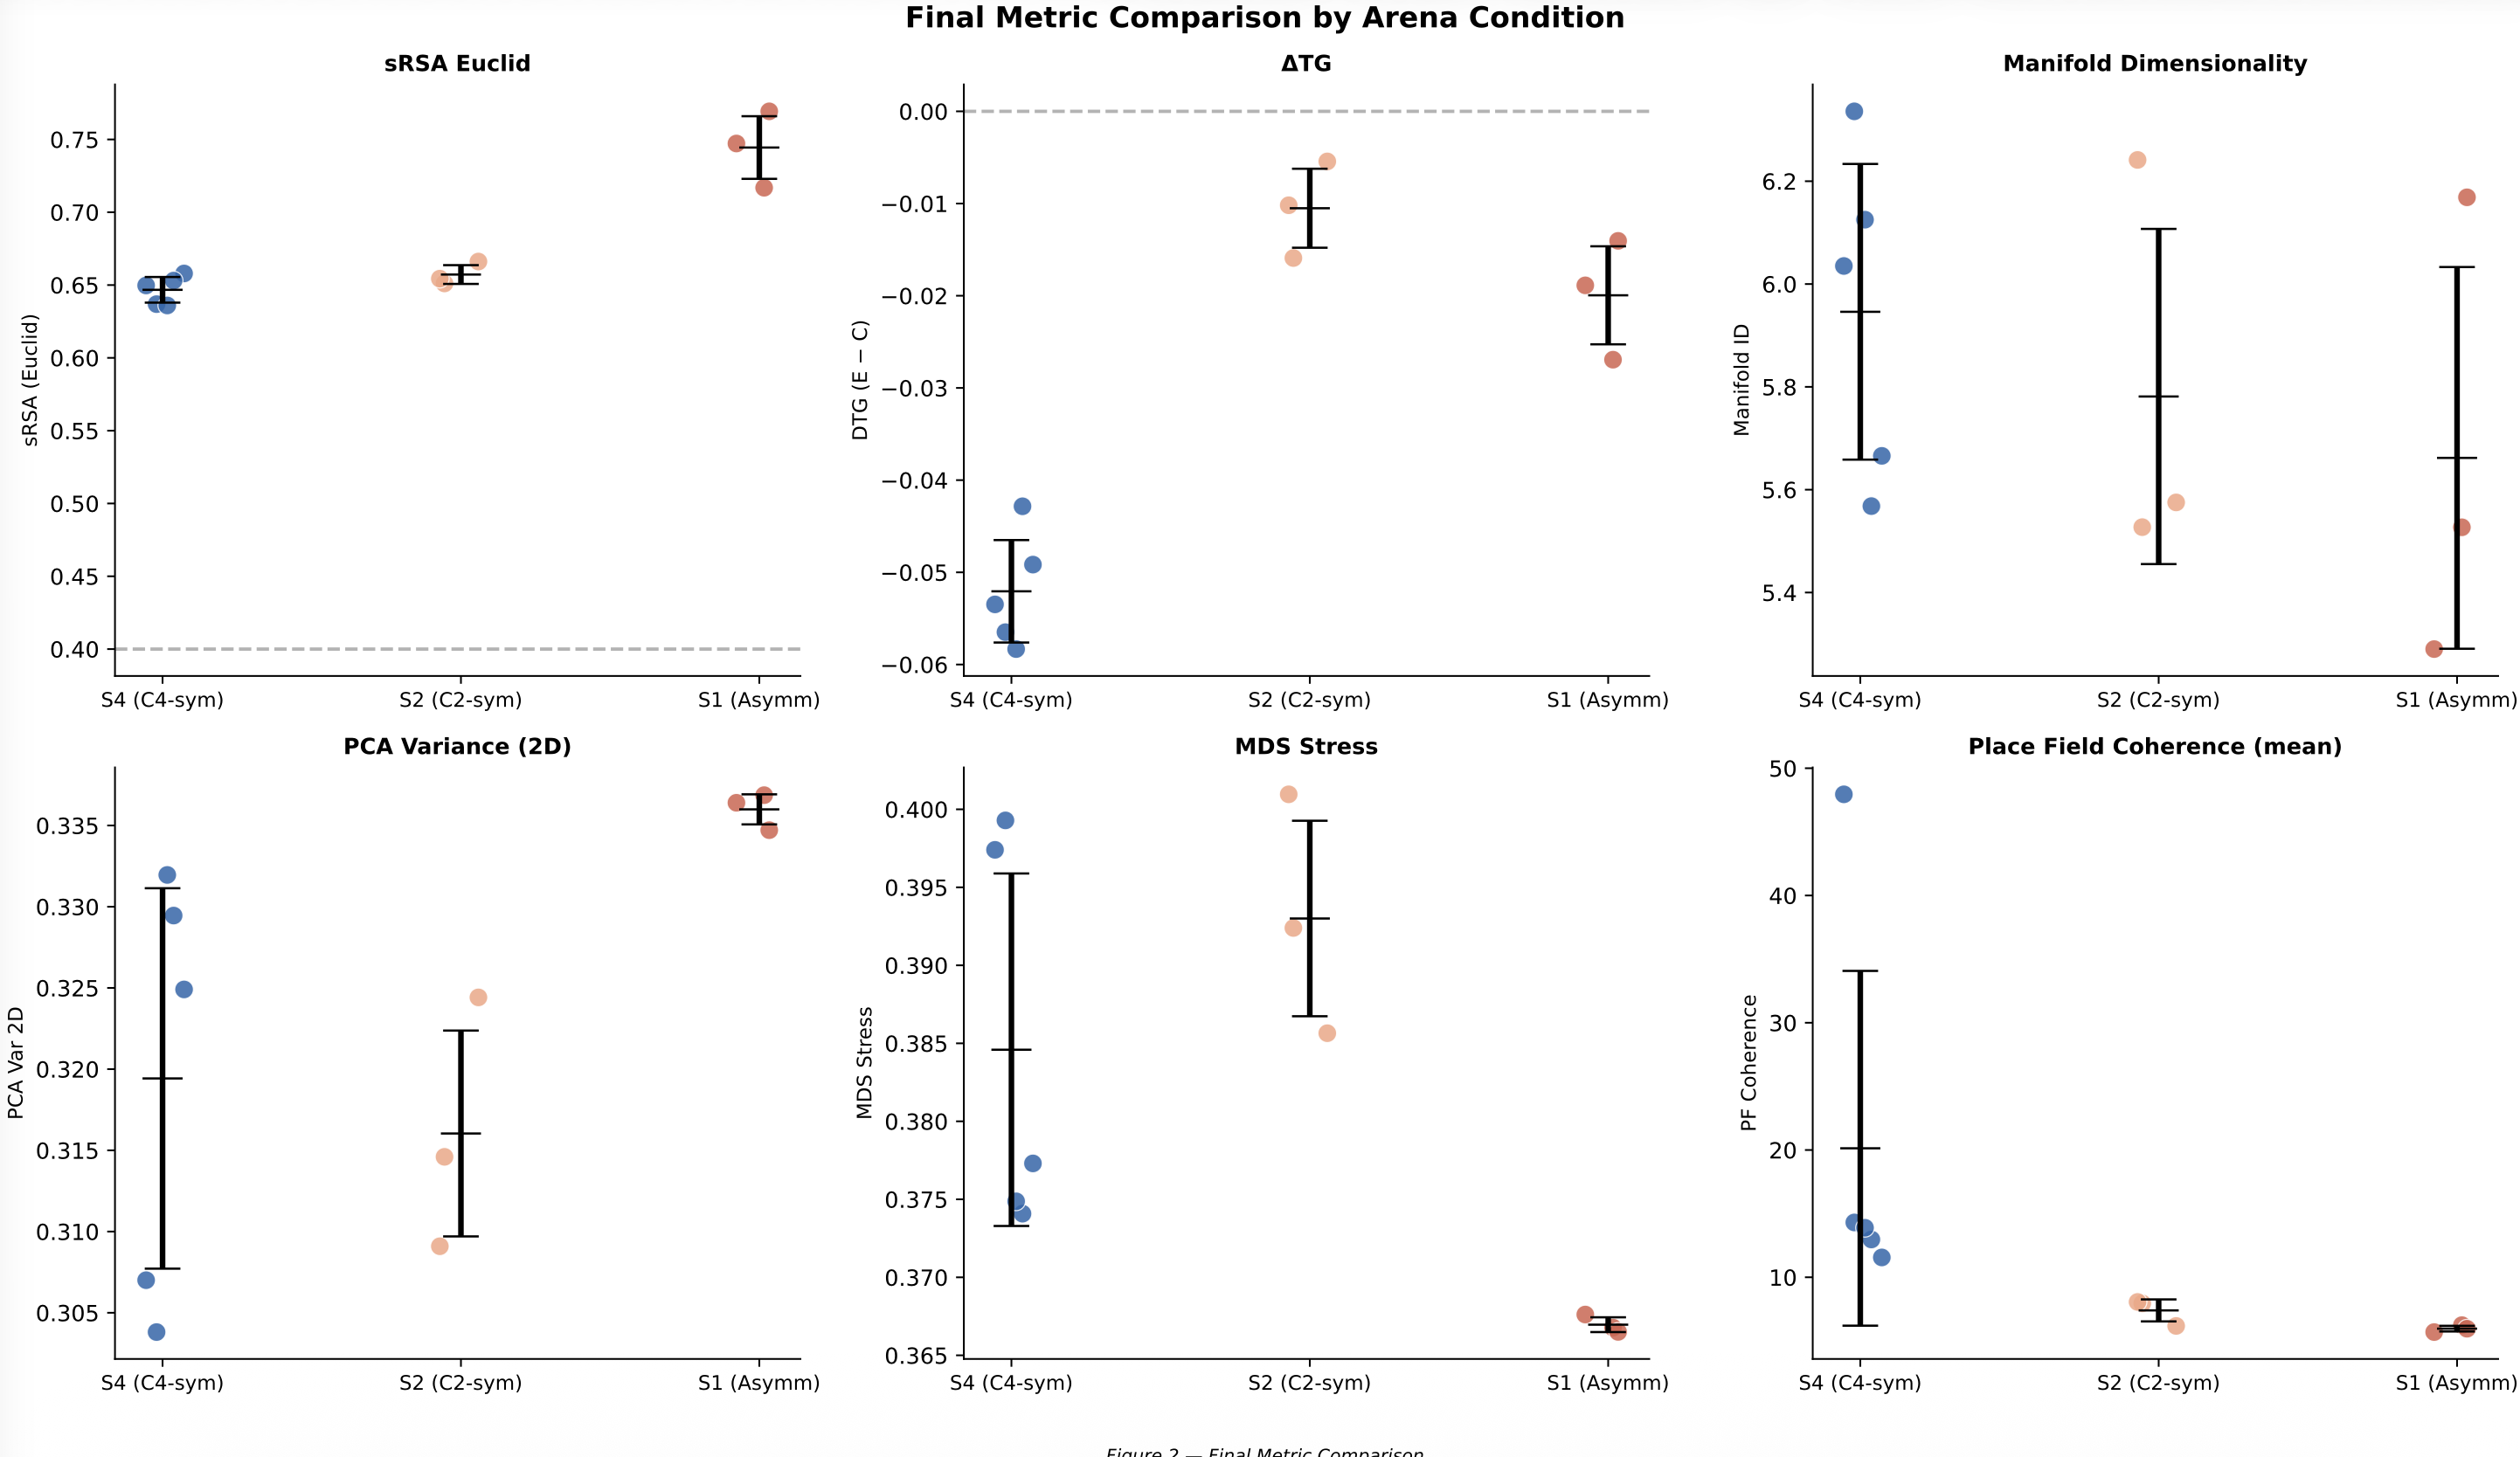
\includegraphics[width=0.64\textwidth]{Dashboardstyleall mertics.png}
\vspace{2pt}
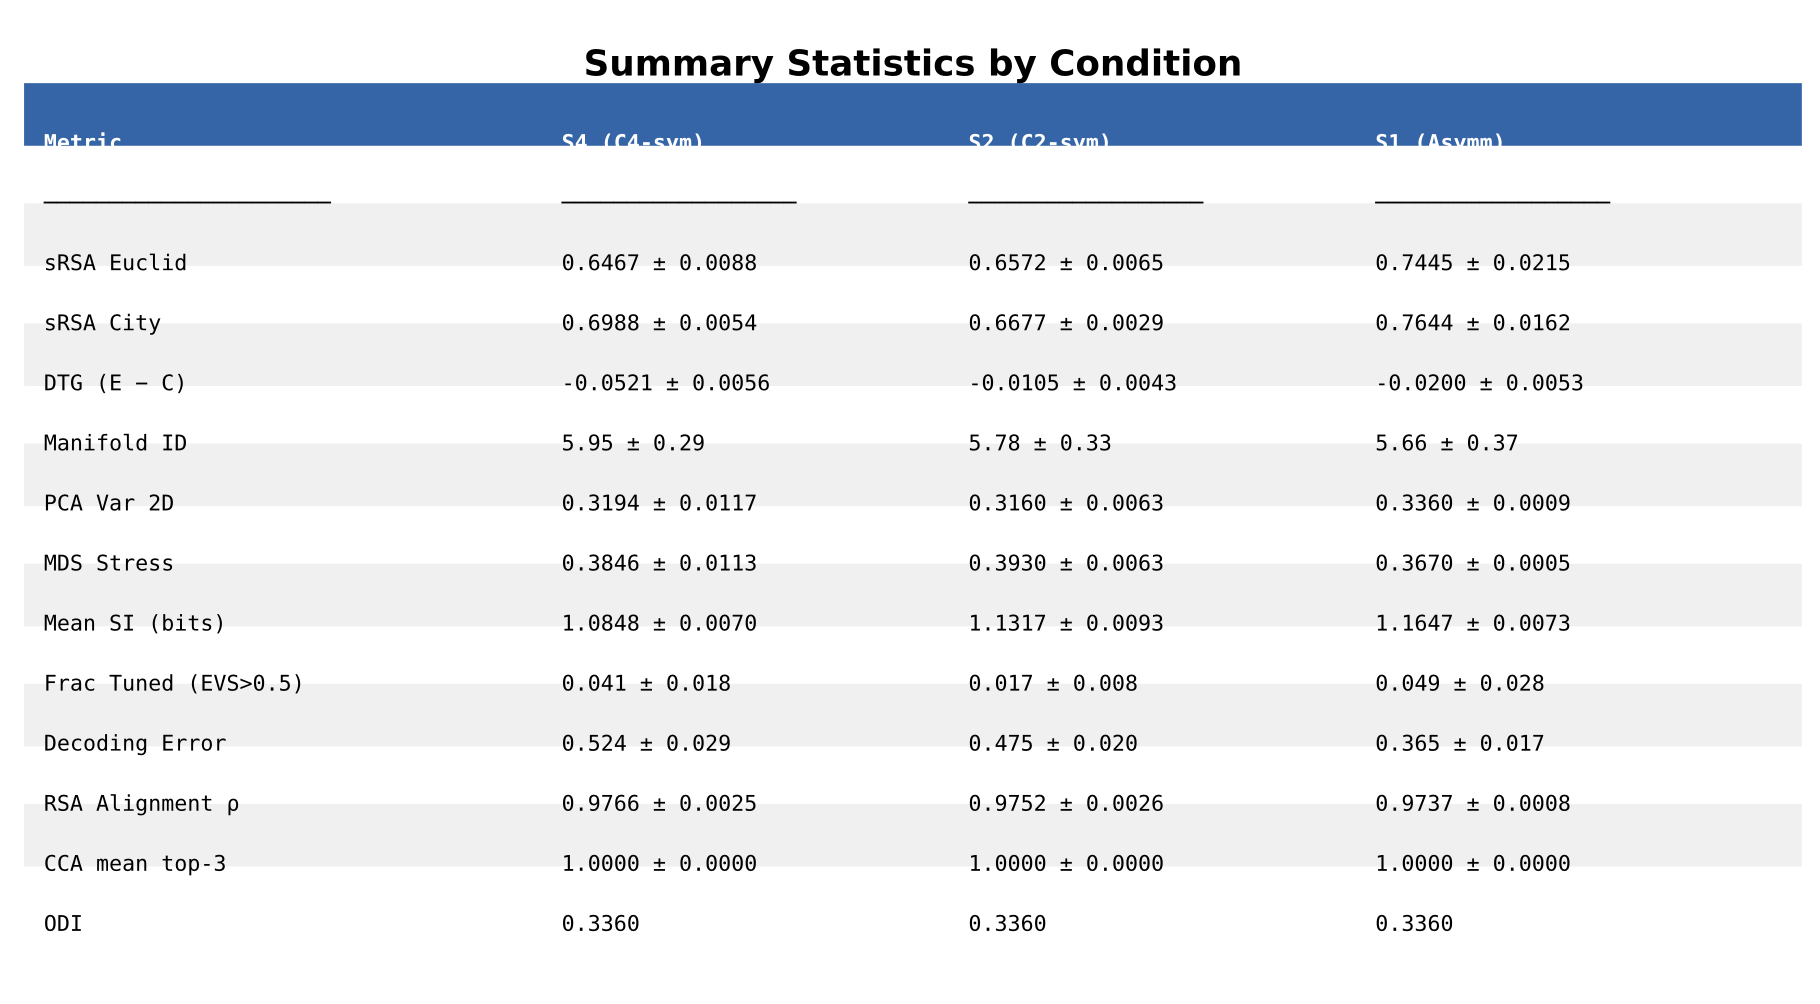
\includegraphics[width=0.50\textwidth]{FInal Table.png}
\refstepcounter{figure}
\label{fig:dashboard}
\label{fig:summarytable}
{\small Figure~\thefigure. Metric overview and summary statistics by condition. S4 has lower map precision, more negative DTG, and higher manifold dimensionality than S1, with ODI fixed at 0.336 in all conditions.}
\end{center}

\subsection{Questions and Evidence Strength}

The strongest results are those tied to a specific mechanism. The monotone decoding error supports equivalence-class folding. The negative S4 $\Delta_{\mathrm{TG}}$ shows that C4 symmetry makes geometry more path-dependent, not more Euclidean. The high cross-seed RSA and low PAA gain reject global orientational degeneracy. The positive C2 Contrast shows that the code respects the observation symmetry group. Weaker evidence includes S2's near-zero $\Delta_{\mathrm{TG}}$ and any fine-grained variance comparison for S2 or S1, because those conditions have only three seeds. Selectivity and spatial-information plots are checks on unit-level coding, not independent proof of the main claim.

\subsection{Decoding Precision Falls With Symmetry}

The decoding result measures usable spatial precision rather than general map structure. A linear decoder read position from the hidden state and was evaluated with city-block tile error. Error increases from S1 to S2 to S4, matching the symmetry group order $|C4|>|C2|>|C1|$ (Figure~\ref{fig:decoding}). In S4, observations at $(x,y)$ are statistically matched by the three $90^\circ$-rotated positions. The recurrent state can partially fold these locations into one equivalence class without increasing prediction loss. A linear decoder then estimates the class centroid, producing an error floor set by within-class spatial spread. S2 has only the $180^\circ$ ambiguity and shows a smaller penalty. This is the most direct evidence that symmetry reduces precision rather than merely changing the visual appearance of tuning maps.

\subsection{Geometry Becomes More City-Block-Biased}

Geometry was evaluated by comparing neural distances against Euclidean and city-block spatial distances. The Distance-Topology Gap is $\Delta_{\mathrm{TG}}=\mathrm{sRSA}_{\mathrm{Euclid}}-\mathrm{sRSA}_{\mathrm{City}}$, so negative values mean city-block distance fits better. All values are negative: S4 $=-0.052$, S2 $=-0.011$, and S1 $=-0.020$. S4 is therefore not more Euclidean; it is the most city-block-biased. Under C4 symmetry, visual observations do not anchor inter-quadrant transitions, so successor geometry generalizes across rotated equivalence classes and path length dominates straight-line distance. The S4 curve continues to diverge through 80,000 steps in Figure~\ref{fig:dtg}, even after final sRSA reaches a comparable map-like value. S2's value of $-0.011$ is anomalously close to zero; with $n=3$ seeds, it should be treated as preliminary rather than as a stable exception.

\begin{center}
\centering
\begin{minipage}{0.44\textwidth}
\centering
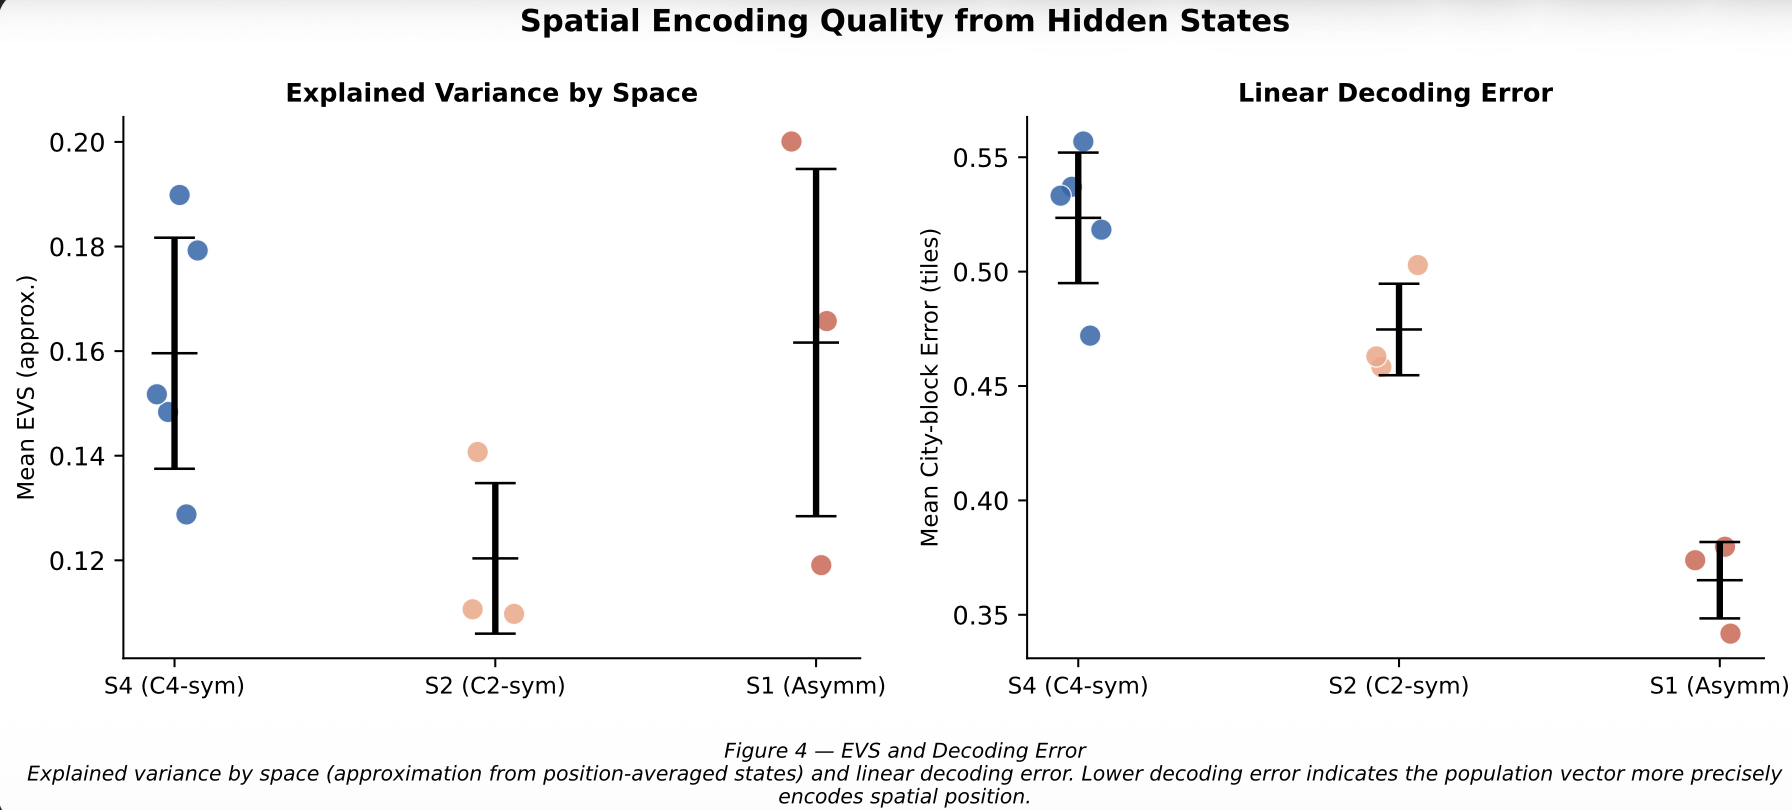
\includegraphics[width=\linewidth]{Decoding_Error.png}
\end{minipage}\hfill
\begin{minipage}{0.46\textwidth}
\centering
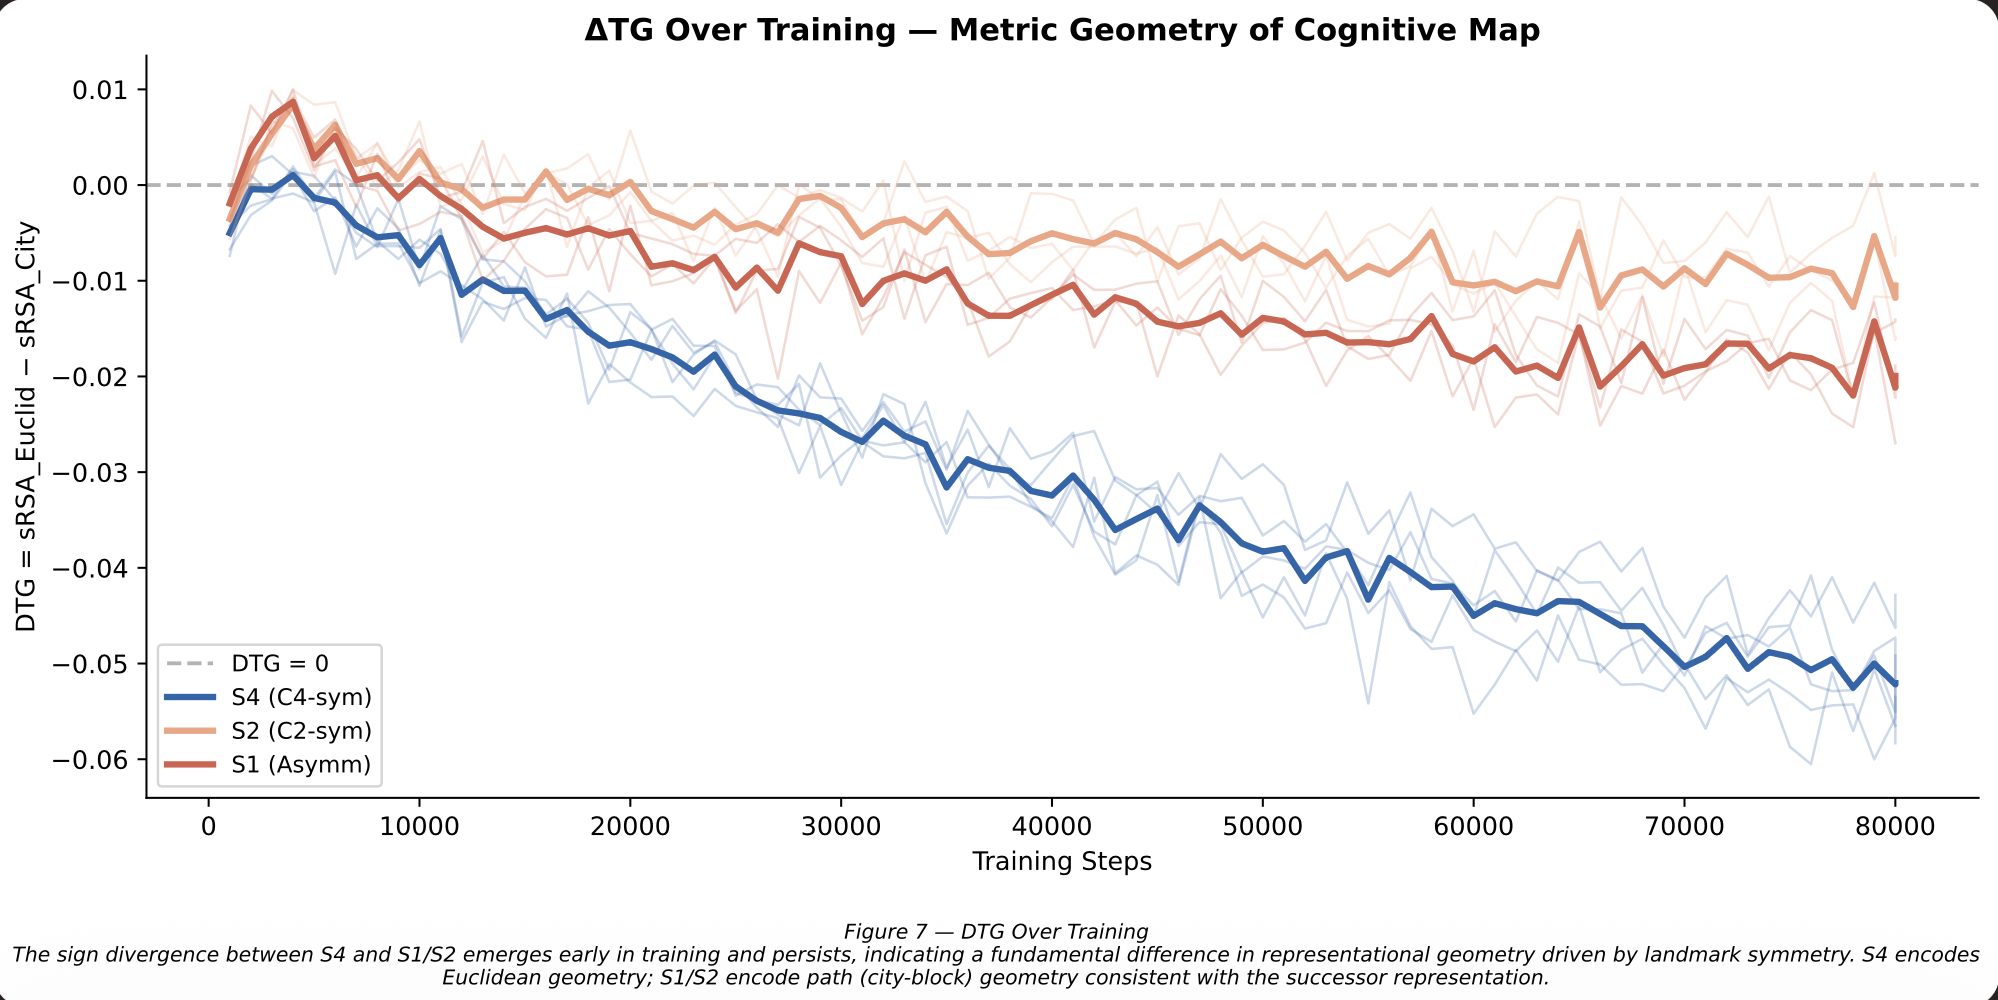
\includegraphics[width=\linewidth]{DeltaTGovertime.png}
\end{minipage}
\refstepcounter{figure}
\label{fig:decoding}
\label{fig:dtg}
{\small Figure~\thefigure. Decoding error and $\Delta_{\mathrm{TG}}$ dynamics. Decoding error rises with symmetry, while negative $\Delta_{\mathrm{TG}}$ indicates stronger city-block than Euclidean fit.}
\end{center}

\begin{center}
\centering
\begin{minipage}{0.45\textwidth}
\centering
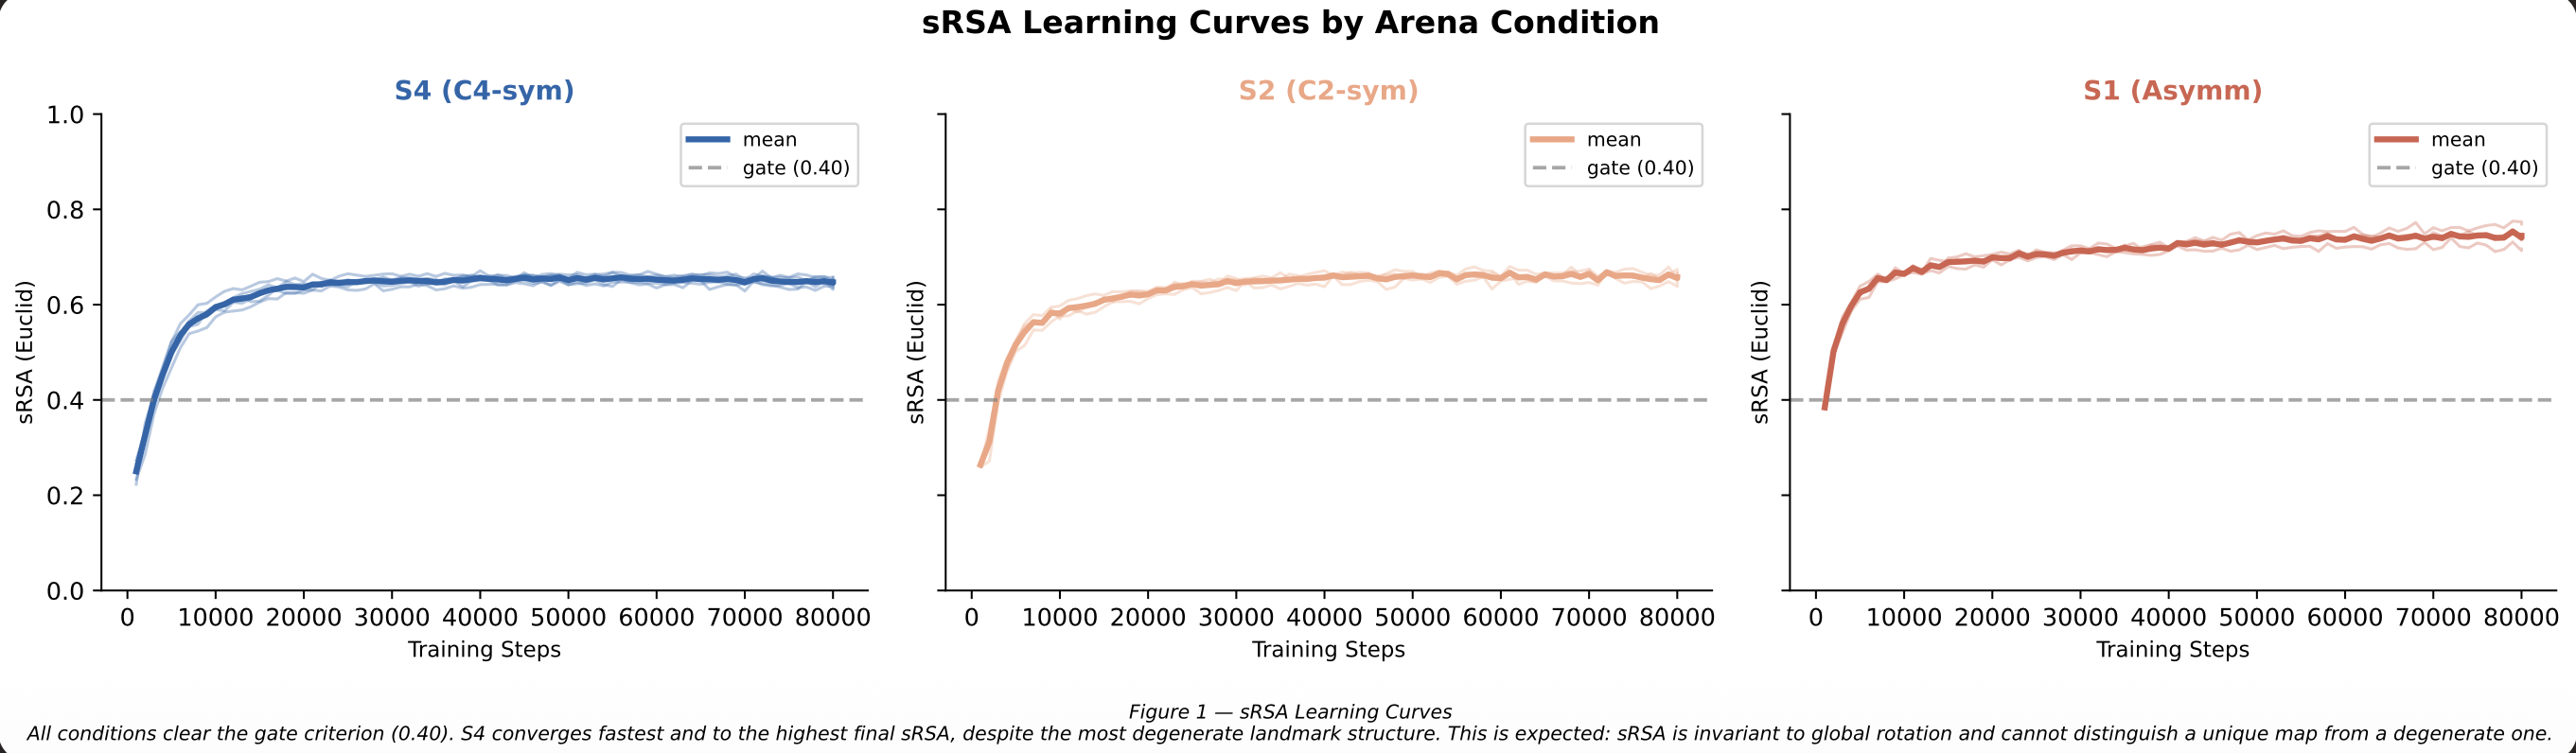
\includegraphics[width=\linewidth]{SRSA.png}
\end{minipage}\hfill
\begin{minipage}{0.45\textwidth}
\centering
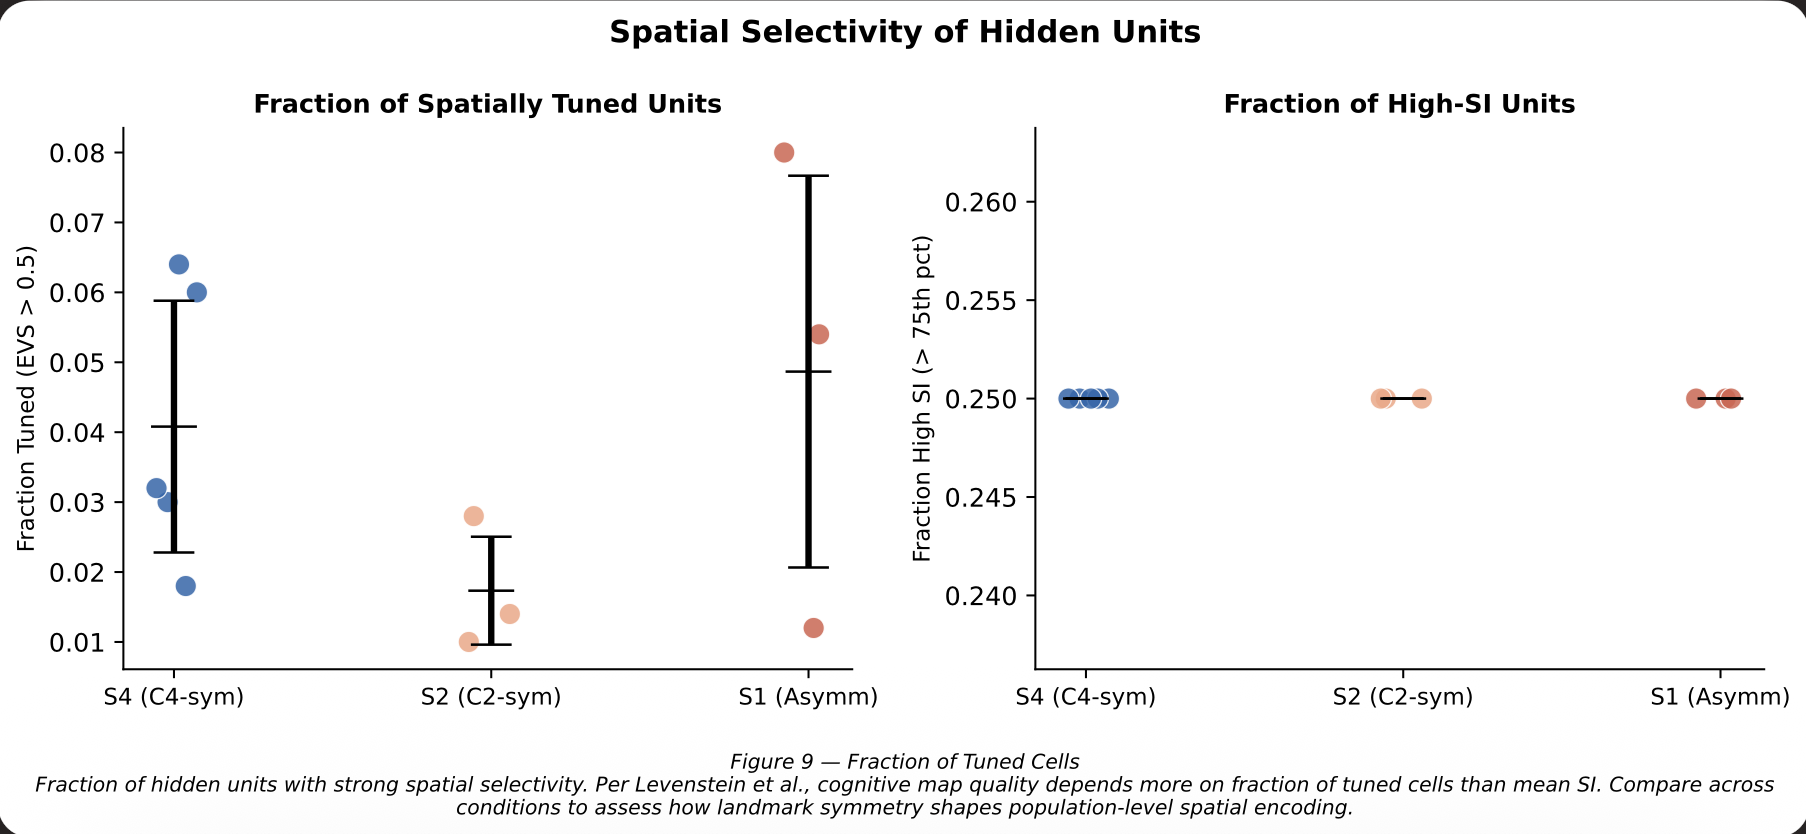
\includegraphics[width=\linewidth]{Spatial_Selectivity.png}
\end{minipage}
\refstepcounter{figure}
\label{fig:srsa_selectivity}
{\small Figure~\thefigure. sRSA and spatial selectivity. sRSA measures map-like pairwise geometry, while selectivity measures how sharply individual units localize.}
\end{center}

\subsection{Degeneracy Is Global-Negative but Local-Positive}

The original degeneracy concern was not supported. Cross-seed RSA alignment stayed high in every condition: S4 $=0.977\pm0.002$, S2 $=0.975\pm0.003$, and S1 $=0.974\pm0.001$ (Figure~\ref{fig:alignment}). PAA asks whether a rotated alignment improves over the identity alignment; its gain was tiny, S4 $=0.006$ and S1 $=0.005$, far below the 0.05 threshold. Independent seeds therefore did not learn incompatible global orientations. The 12-bin head-direction input provides the most direct explanation: it breaks rotational equivalence in the transition sequence even when the visual observation function is C4-symmetric.

Local aliasing did increase. Rotational autocorrelation compares a unit's tuning map with its rotated copies; it was S4 $=0.187$ versus S1 $=0.069$, a 2.7$\times$ elevation. The four-peak unit fraction also increased, from 4.5\% in S1 to 7.7\% in S4. The failure mode is local folding, not global collapse. Individual units can repeat responses at symmetric positions while the population as a whole keeps a shared global orientation.

\begin{center}
\centering
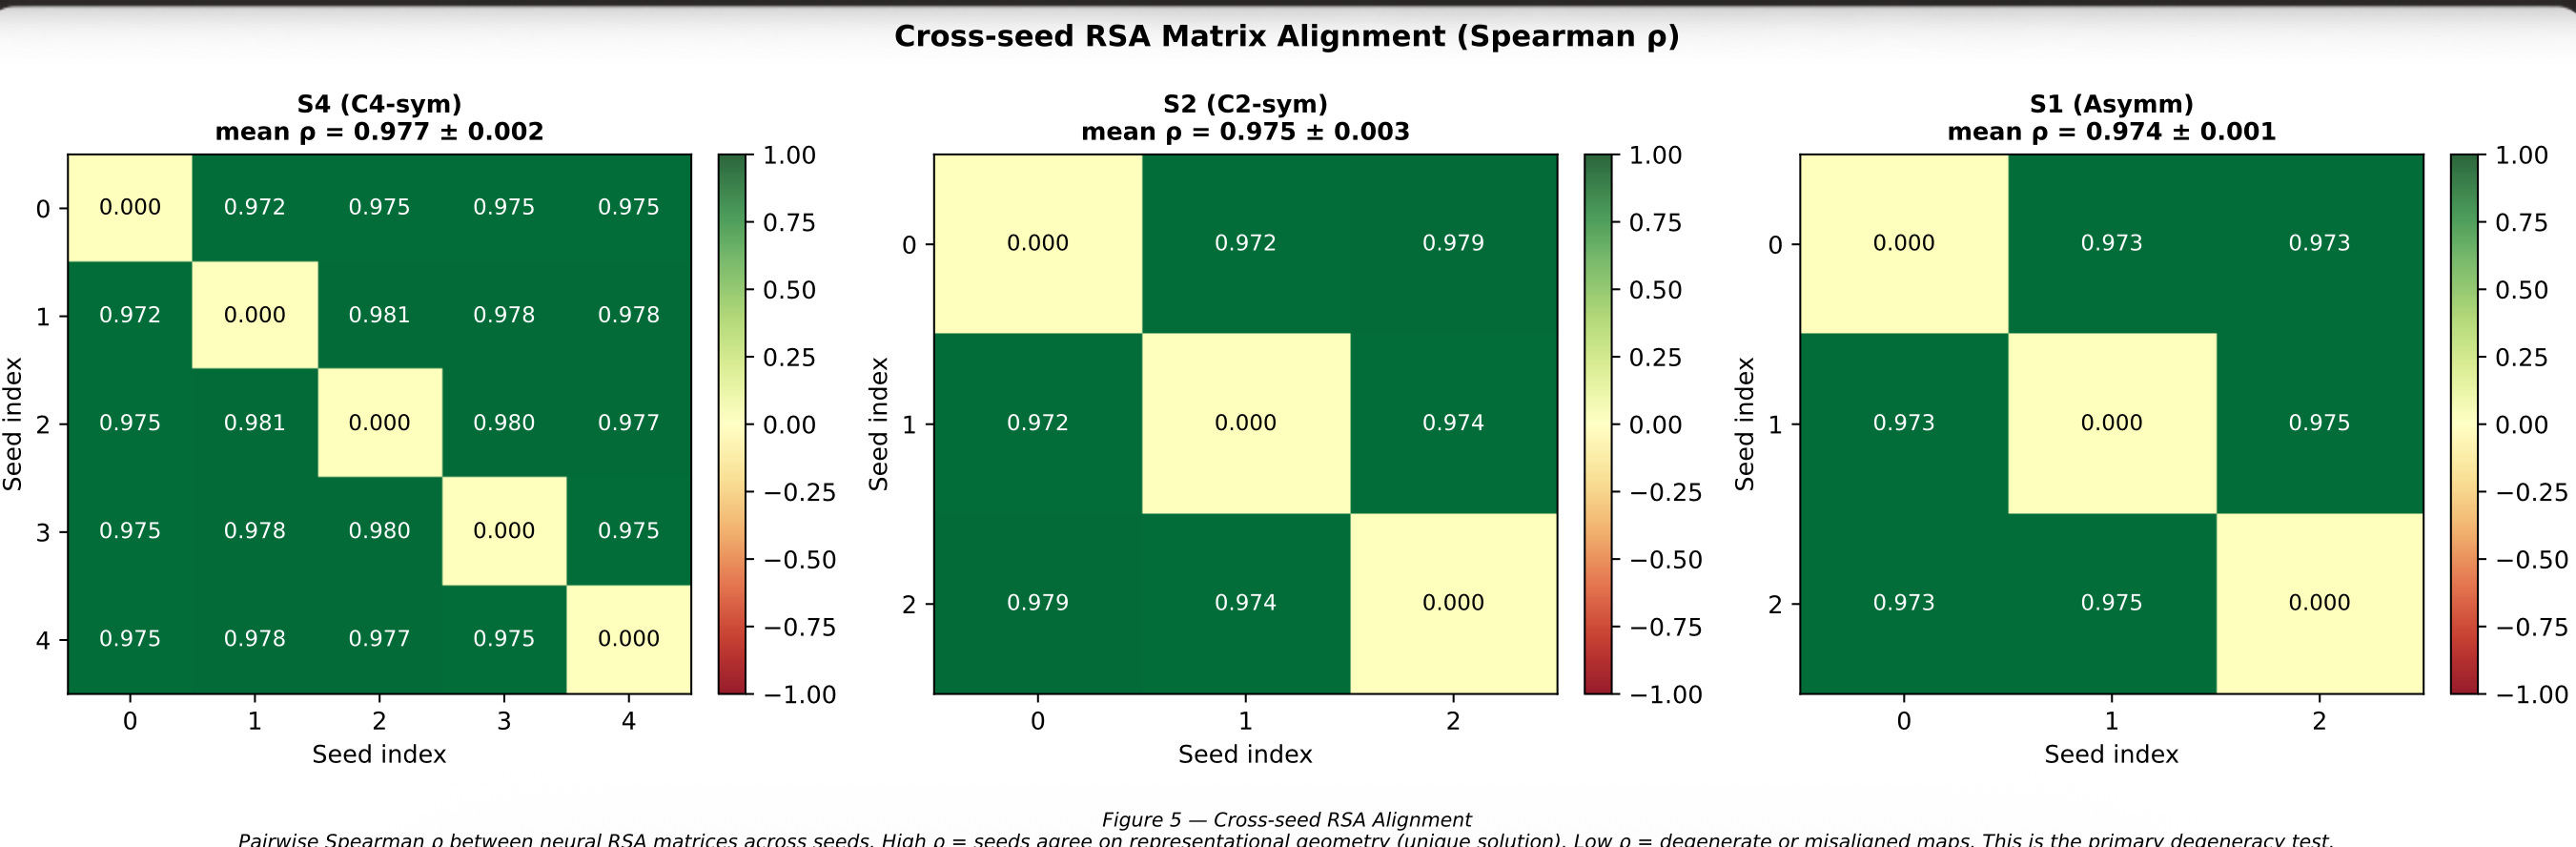
\includegraphics[width=0.74\textwidth]{Correlationperexperiment.png}
\refstepcounter{figure}
\label{fig:alignment}
{\small Figure~\thefigure. Cross-seed RSA alignment matrices. High off-diagonal correlations in all conditions show that global map geometry is reproducible across seeds.}
\end{center}

\subsection{C2 Symmetry Is Encoded in the Population Code}

C2 Contrast was S4 $=-0.130$, S2 $=+0.045$, and S1 $=-0.070$. The contrast compares similarity for $180^\circ$-related quadrant pairs against $90^\circ$-related pairs. A positive value means that the population treats the C2-equivalent quadrants as more similar. This is exactly the relation imposed by the S2 observation function. The result cannot be reduced to generic precision loss, because generic loss would blur all quadrant distinctions rather than selectively favoring the C2-equivalent pairs. The network had no group-theoretic objective; this structure emerges from prediction over symmetric observation sequences.

\subsection{Symmetry Raises Manifold Dimensionality}

TwoNN dimensionality was S4 $=5.95\pm0.29$, S2 $=5.78\pm0.33$, and S1 $=5.66\pm0.37$. This is opposite the simplest collapse prediction. A folded code does not become a cleaner low-dimensional quotient; it uses extra dimensions to retain partial path-history distinctions among visually equivalent positions. PCA Var(2D) is higher in S1 than S4, 0.336 versus 0.319, and MDS stress is lower in S1 than S4, 0.367 versus 0.385. The manifold result explains why decoding can worsen even when sRSA remains nontrivial: the representation is spatial, but its geometry is less accessible as a clean two-dimensional map. Figure~\ref{fig:unit_id} shows the spatial-information and dimensionality measures.

\begin{center}
\centering
\begin{minipage}{0.45\textwidth}
\centering
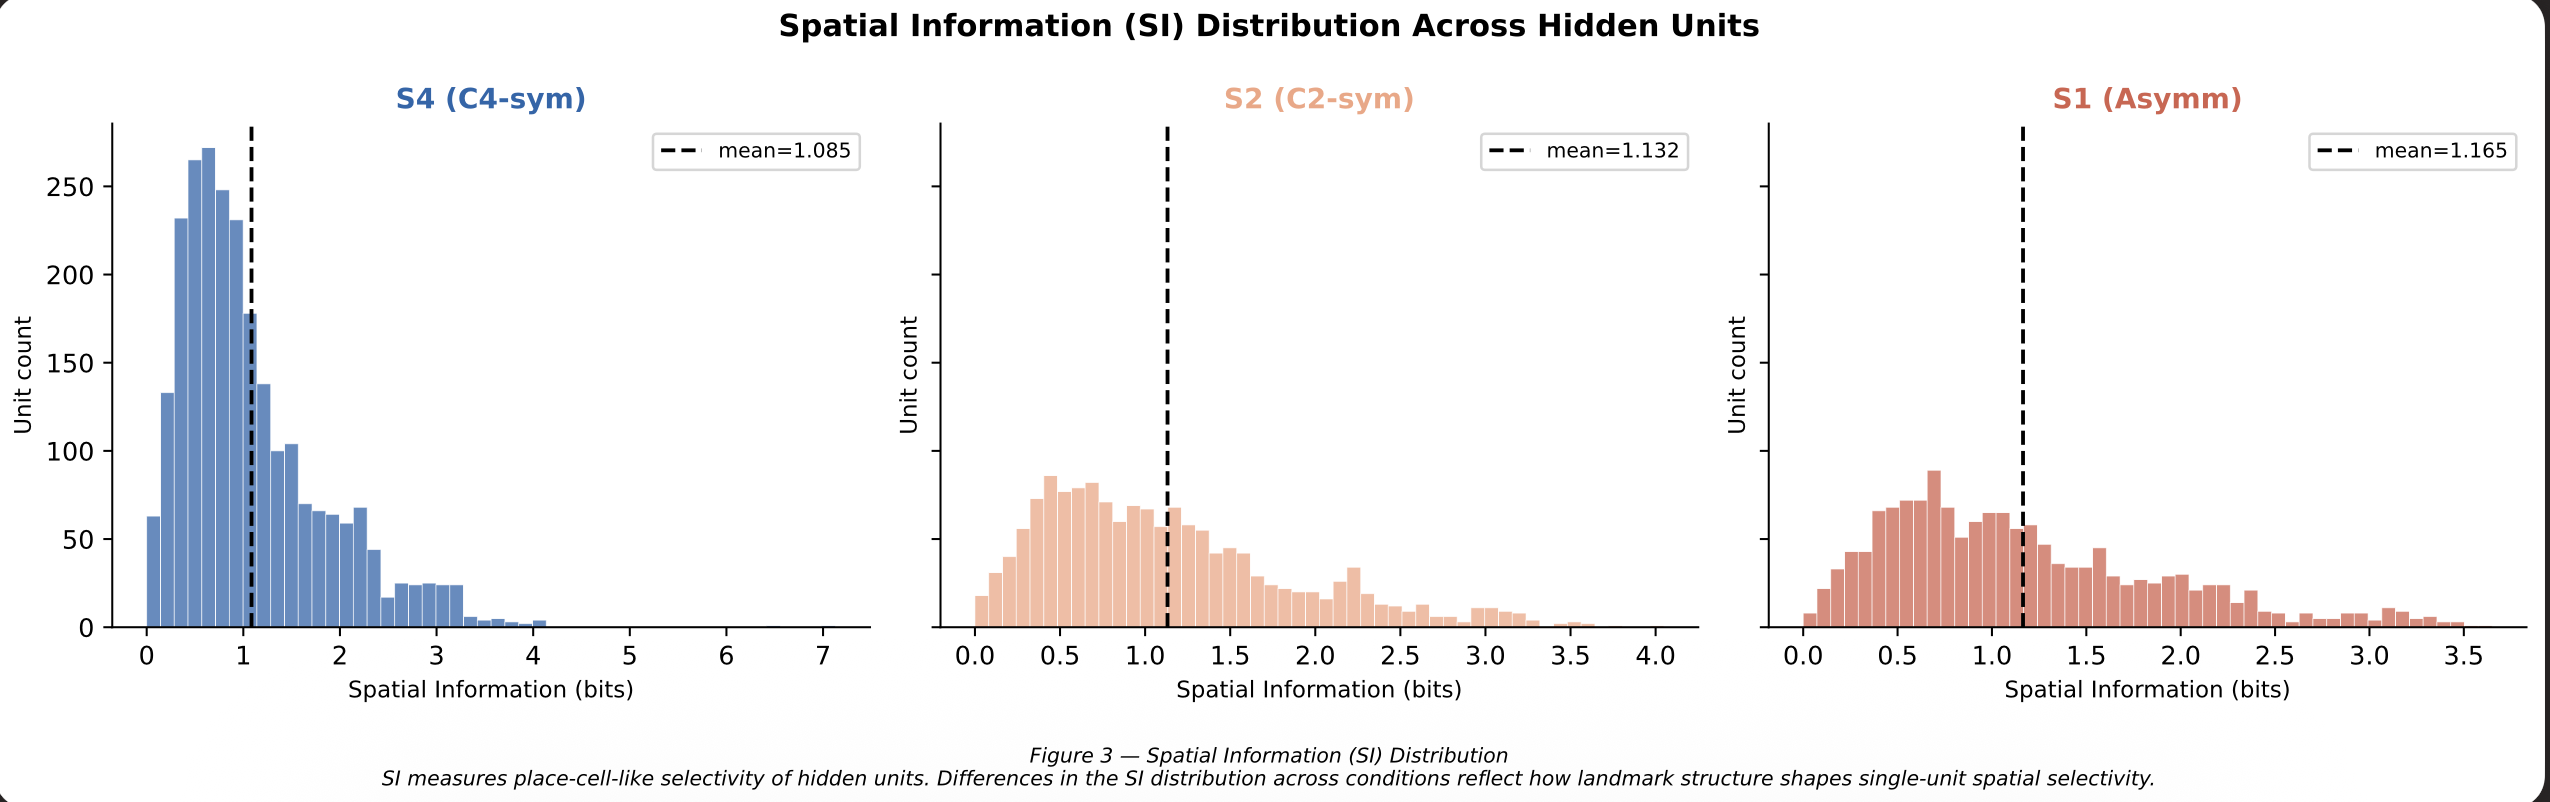
\includegraphics[width=\linewidth]{SI.png}
\end{minipage}\hfill
\begin{minipage}{0.45\textwidth}
\centering
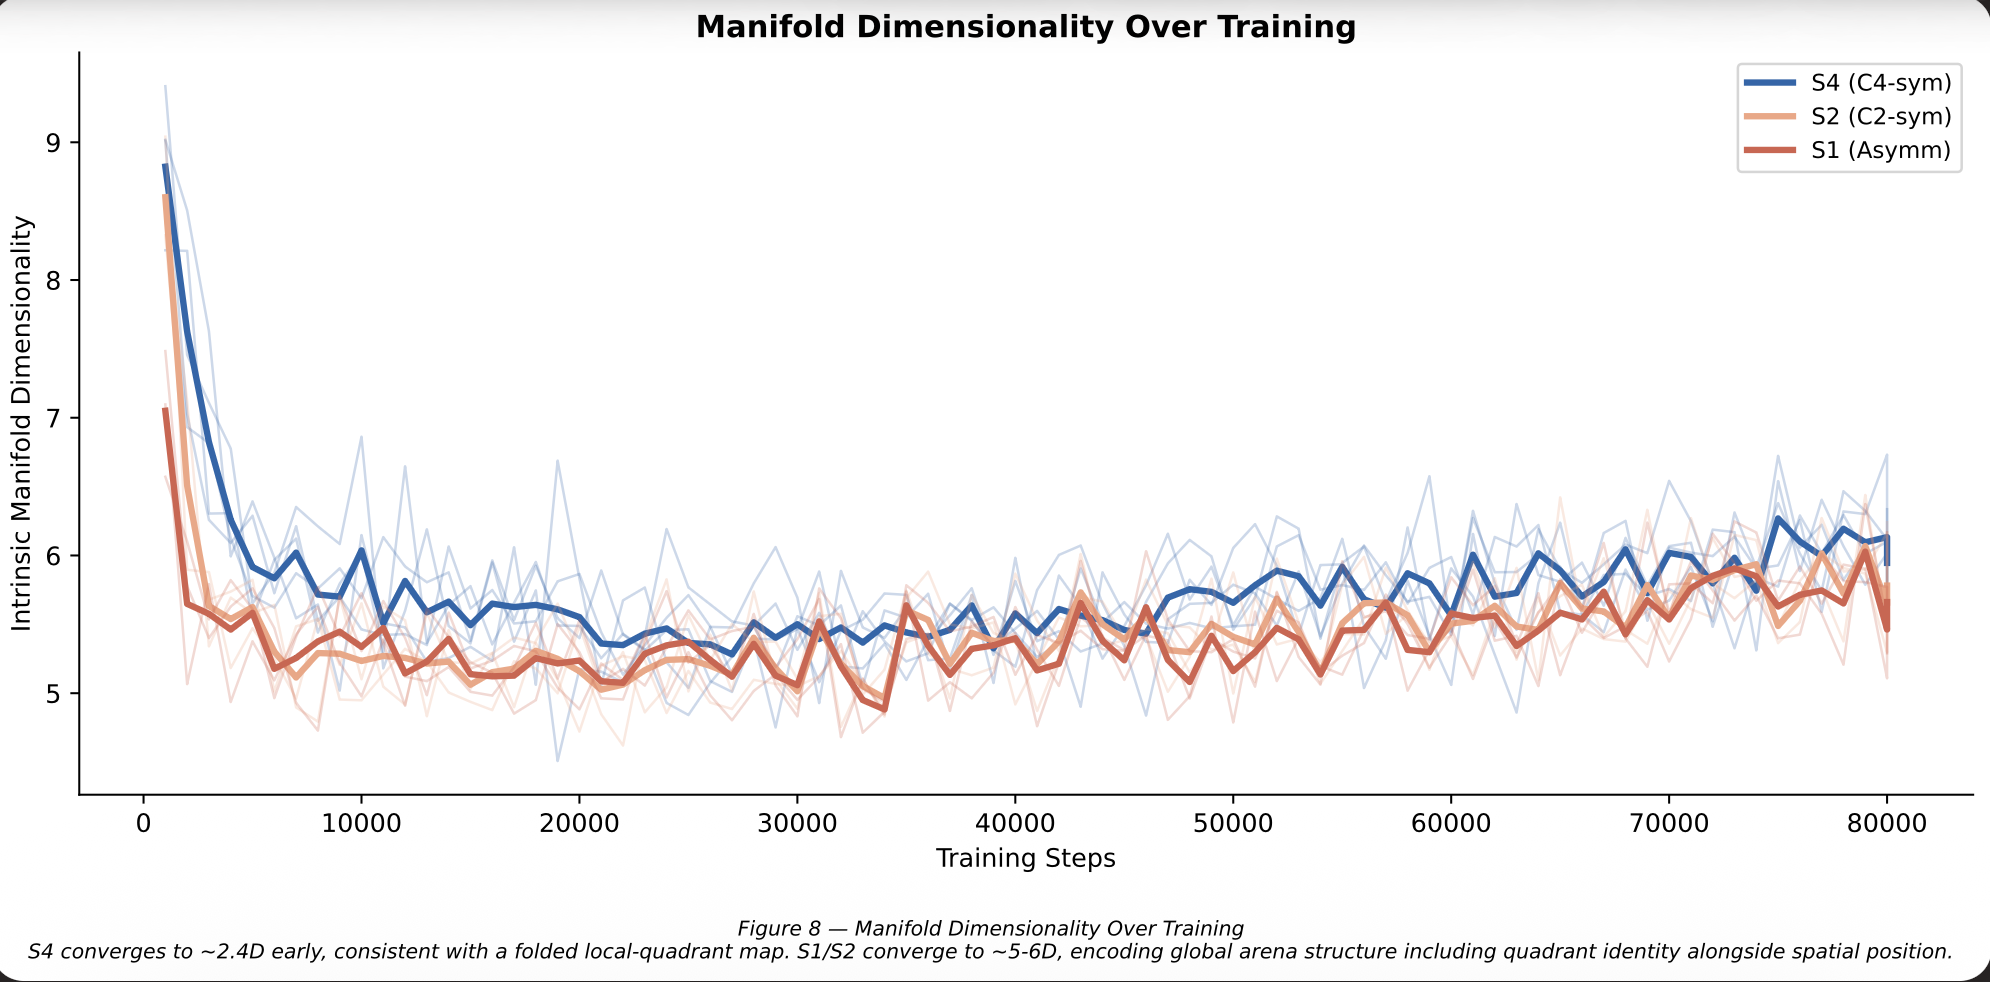
\includegraphics[width=\linewidth]{ID_overtime.png}
\end{minipage}
\refstepcounter{figure}
\label{fig:unit_id}
{\small Figure~\thefigure. Spatial information and TwoNN dimensionality. S4 ends with higher dimensionality, consistent with path-history structure rather than simple representational collapse.}
\end{center}

\section{Discussion}

Landmark symmetry produces precision loss, local aliasing, and a more path-biased geometry, but not global orientational degeneracy. This reframes the reason to avoid symmetric arenas in predictive-map experiments. The map does not disappear under C4 symmetry; it becomes less spatially precise and less faithful to geometry. sRSA alone misses this distinction because it can remain high while decoding worsens, $\Delta_{\mathrm{TG}}$ drifts, and single units become rotationally aliased.

The head-direction input explains why global orientation can survive. Visual observations are symmetric, but trajectories are not purely visual: direction and action provide an oriented transition signal. This separates two sources of information. Landmarks determine which positions are visually confusable, while head direction constrains how the state evolves through those positions. A C4 visual layout can therefore produce local aliasing without allowing the entire population map to rotate freely across seeds.

The C2 result addresses a different mechanism. Predictive learning can encode the actual symmetry group of the observation function, not just a noisy or blurred spatial map. In S2, the positive C2 Contrast means that the network specifically groups $180^\circ$-related quadrants. This organization is too structured to be explained by generic imprecision. It indicates that the recurrent state is shaped by the equivalence relation that governs future observations.

Three limitations remain. Three seeds for S2 is insufficient to establish whether the anomalous DTG value ($-0.011$) reflects a real departure from monotone ordering or sampling variance; this result should be treated as preliminary. The PAA degeneracy threshold of 0.05 is heuristic; a continuous degeneracy measure, such as SCI, would remove the arbitrary threshold dependency. The $18\times18$ discrete MiniGrid environment imposes a city-block navigation metric by construction; the DTG result may partly reflect this environmental structure rather than purely representational geometry, and should be replicated in a continuous environment. The defensible conclusion is strongest for decoding precision, DTG sign, cross-seed alignment, and C2 Contrast; selectivity and spatial information support the same interpretation but should not carry the argument alone.

\section{Conclusion}

Overall, landmark diversity matters because it anchors predictive transitions that distinguish otherwise equivalent locations. Symmetry does not destroy the learned cognitive map, but it folds it, lowers readout precision, and can imprint group structure directly into the population code.

\bibliographystyle{plainnat}
\bibliography{references}

\end{document}
